\documentclass[article,english,colorback,accentcolor=tud9b,11pt]{tudreport}
%\documentclass[ngerman,longdoc,colorback,accentcolor=tud9b,11pt]{tudreport}

%% Versionierung: %%%%%%%%%%%%%%%%%%%%%%%%%%%%%%%%%%%%%%%%%%%%%%%%%%%%%%%%%%%%%%%%
%
\newcommand{\version}{2012.001}
%%%%%%%%%%%%%%%%%%%%%%%%%%%%%%%%%%%%%%%%%%%%%%%%%%%%%%%%%%%%%%%%%%%%%%%%%%%%%%%%%%


%%%%%% PRESETTINGS

\usepackage{babel}
\usepackage{listings}										%Programmcode einbinden
\usepackage{tikz}
\usetikzlibrary{decorations.pathreplacing}
\usepackage{amsmath}
\usepackage{hyperref}

\usepackage[numbered,framed]{mcode}			%Matlabcode einbinden

\title{Octave Interface for Onelab}
\subtitle{Alexander Krimm}
\institution{Institut für Theorie elektromagnetischer Felder\\TU-Darmstadt}
\date{\today}

\sponsor{%
\begin{minipage}{0.47\textwidth}
  Stand: \today
\end{minipage}
%\begin{minipage}{0.47\textwidth}
% \flushright{\textbf{SS 2014}}
%\end{minipage}
}

\setinstitutionlogo{TEMF-Logo}


\begin{document}
	
    \maketitle
%    \setcounter{tocdepth}{3}
%    \setcounter{secnumdepth}{3}
%    \tableofcontents

		\begin{abstract}
			Open Numerical Engineering LABoratory (ONELAB)\footnote{\url{http://onelab.info/}} is a project that aims to simplify the use of various Finite Element Software by providing a client/server based Protocoll for different solvers to exchange data. Non-native clients can be used by wrapping their input data and the calls to them into *.ol files, but it is more comfortable for the solvers to interface directly with the ONELAB server. The reference server is included in the meshing software Gmsh\footnote{\url{http://www.geuz.org/gmsh/}} and includes C++ Headers and a Python module. The goal of the Octave Interface for ONELAB is to provide similar functionalities for solvers written in octave\footnote{\url{http://www.gnu.org/software/octave/}}, as many solvers are written in an Octave compatible language.
		\end{abstract}

		\section{Installation}
		\subsection{Installation from Octave Package}
		If you've got the \texttt{onelab-?.?.?.tar.gz} you can install it from octave by running:
		\begin{lstlisting} 
			pkg install onelab-?.?.?.tar.gz
		\end{lstlisting}
		This installs the octave Package into your home directory or if you've got the necessary privileges into the respective global directory.

		\subsection{Compilation from Source}
		ONELAB comes with a small Makefile, so on unixoid systems a simple \texttt{make all} in the \texttt{src} directory should do the job. To use the octfile compiled this way you have to add your build directory to the octave-path with \texttt{addpath}.

		\subsection{Generating the Octave package from source}
		If you want to change things in the code and install your modified version as an octave package you can build one with \texttt{make pkg}. Be sure to run \texttt{make clean} before. The files in the parent directory of src are also important for building the package.
		
		\section{Usage}
		To use ONELAB in octave make sure you have a recent Gmsh version\footnote{The Version used to test this was 2.8.4} and the package is installed somewhere octave can find it.
		\subsection{Setting up the connection}
		To execute an Octave m-file with ONELAB you have to add it as a solver within the Gmsh interface via ``add solver'', see Fig.~\ref{fig:gmsh}. Since ONELAB will call the script as an executable the script must start with a proper shebang:
		\begin{lstlisting} 
			#!/usr/bin/octave -qf
		\end{lstlisting}
		When added and every time you click on the ``run''-button Gmsh will initialize the script. To establish the connection your script has to read out where to connect from the options and open the connection with the \texttt{ol\_connect} command.
		\begin{figure}[b]
			\centering
			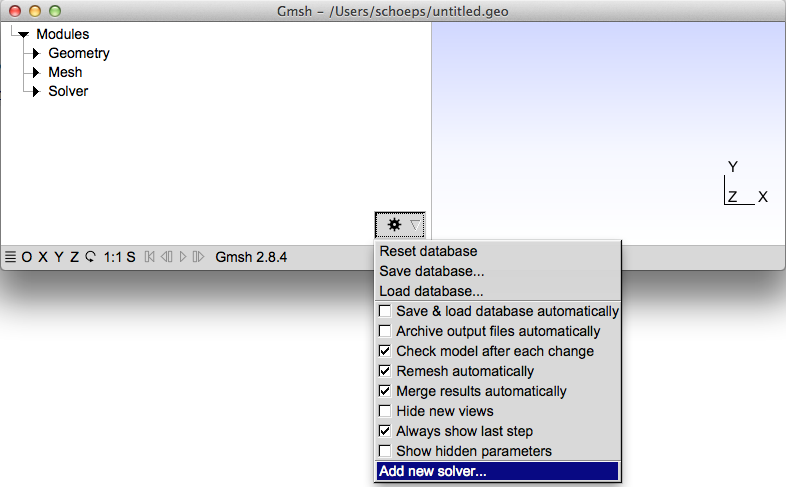
\includegraphics[width=.4\textwidth]{gmsh.png}
			\quad
			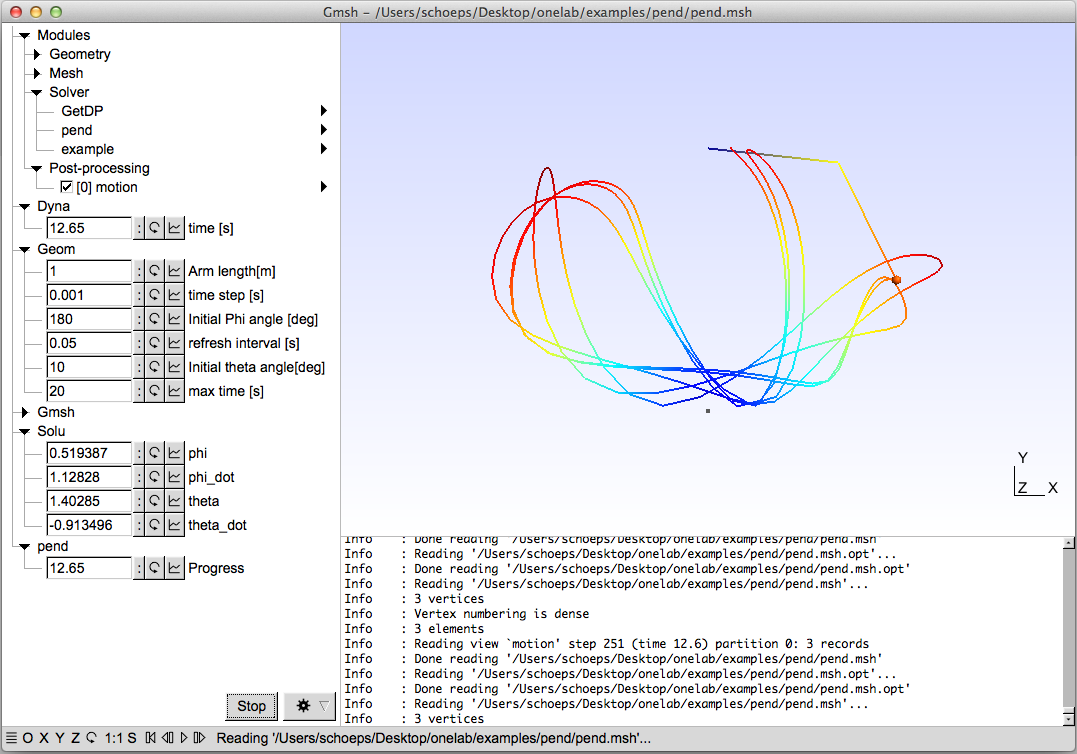
\includegraphics[width=.4\textwidth]{pend.png}        
			\caption{Add a solver in Gmsh and screenshot of the pendulum solver (on Mac OS X)}
			\label{fig:gmsh}
		\end{figure}
		\begin{lstlisting} 
% load the ONELAB api
pkg load onelab;
% parameter parsing
for i = [1:nargin]
  if (i+2 > nargin)
    error('invoke with -onelab name server_addr');
  elseif (strcmp(argv({i},'-onelab'))
    name = argv({i+1};
    addr = argv({i+2};
    break;
  endif
endfor
% Start the client
ol_client(name, addr);
		\end{lstlisting}
		To find out what is expected from our solver we have to read out the ``Action'' parameter from ONELAB, for example with:
		\begin{lstlisting} 
% Quit if the requestet action is not to compute
action = ol_getParameters([name '/Action']);
if (!strcmp(action{1}.value, 'compute'))
	printf('Nothing to do');
	ol_disconnect()<++>;
	exit;
endif
		\end{lstlisting}
		Before exiting the script should properly close the connection with:
		\begin{lstlisting} 
ol_disconnect();
		\end{lstlisting}

		\subsection{Reading and Writing Parameters}
		To read parameters from ONELAB the package provides the \texttt{ol\_getParameters} command. If called without argument it returns all parameters from the server, if called with a parameter name, it returns just that parameter or an empty list. Note that the function always returns cell arrays, so you have to index them with \texttt{\{i\}} even if just one element is returned. The parameters itself are represented as maps, the most important keys are name, value, type, label, help and choices.

		To write parameters you can call the function \texttt{ol\_setParameter} either with a single parameter containing a structure like the one returned by \texttt{ol\_getParameters} where the fields name, value and type are mandatory or with more parameters name, type and value.
		\subsection{Launching Subclients}
		If you want to use other software from inside your solver ONELAB allows you to launch ``subclients''. They can be either blocking or non-blocking:
		\begin{lstlisting} 
% run subclient and wait until it is finished before continuing
ol_runBlockingSubClient('subclient', ...
'getdp ReadPoint.pro -res LaplacianNeumann.res -pos readPoint');
% run other subclient
ol_runNonBlockingSubClient('subclient2', ...
'super-cool-simulation-software -solve -real -fast');
% do some stuff
ol_waitOnSubClients();
% do someting with the results and exit
		\end{lstlisting}
		The first parameter is the name the subclient gets passed and is also prepended to it's debug output in the Gmsh console.

		\subsection{Other useful commands}
		Other useful commands are mostly for logging:
		\begin{lstlisting}
% show a red error in the ONELAB console 
ol_sendError('something went wrong')
% show informative output in the ONELAB console
ol_sendInfo('hey there')
% show warnings in the ONELAB console
ol_sendWarning('this looks strange')
% display progress in the Gmsh status bar
ol_sendProgress('reading file: input.txt')
		\end{lstlisting}

		You can also send a Merge File request to force Gmsh to read and display msh files:
		\begin{lstlisting}
ol_sendMergeFileRequest('foo.msh');
		\end{lstlisting}

		\subsection{Interactive use}
		Often when you have computation intensive calculations running you want to check if the results can be right while the computations are still running. You can use ONELAB from the octave terminal to do exactly that. Just use \texttt{interactive.m} as a solver and start your regular solver with \texttt{ol\_runNonBlockingSubClient}. While this works on some systems you might have to modify the \texttt{interactive.m} script to lauch the right terminal and respect the escaping rules of your shell.
		\section{Examples}
		The octave ONELAB package ships currently with two examples, one being a simple standalone simulation of a pendulum, the other example is using GetDP as a subclient and reading back field values from it.
		\subsection{pend.m}
		Just run the solver by adding it from within Gmsh and after clicking run it will visualize the movement of the pendulum and export values for the angles for the time steps, see Fig.~\ref{fig:gmsh}. You can then visualize them over the time.
		\subsection{LaplacianNeumann}
		This solver shows the use of subclients to exchange data between octave and other ONELAB solvers. The problem is a simple Laplacian problem on the unit square. The excitation can be varied with a ONELAB parameter. This whole problem is described in the LaplacianNeumann.pro file. The octave solver \texttt{example.m} calls GetDP\footnote{\url{http://geuz.org/getdp/}} on this problem with different parameter values. Another call to GetDP is made to export the values of specific points to ONELAB, as specified in the ReadPoint.pro file. The octave script then reads the value of these 2 points and multiplies their values returning the result to another ONELAB parameter. 

		\section{License}
		The code is licensed under the LGPL v3 or later\footnote{\url{http://www.gnu.org/licenses/lgpl.html}}.
\end{document}
